\section{Method}
\label{sec:method}

Let us formulate calibration as a trajectory-conditioned inverse problem.  Let
$z_t$ denote the simulated particle state, $u_t$ the measured poses and
velocities of the two spatulas, $\theta$ the fitted material parameters, and
$\psi$ the fixed reconstruction, contact, camera, and numerical settings:
\begin{equation}
\begin{aligned}
z_{t+1} &= \mathcal{S}_{h,\Delta t}(z_t,u_t;\theta,\psi),\\
y_t &= \mathcal{H}_{c}(z_t)+\delta_t+\epsilon_t .
\end{aligned}
\label{eq:inverse_problem}
\end{equation}
% \begin{equation}
%  z_{t+1}=\mathcal{S}_{h,\Delta t}(z_t,u_t;\theta,\psi),\qquad
%  y_t=\mathcal{H}_{c}(z_t)+\delta_t+\epsilon_t .
%  \label{eq:inverse_problem}
% \end{equation}
Here $\mathcal{H}_{c}$ projects particles into the calibrated depth camera,
while $\delta_t$ and $\epsilon_t$ denote model discrepancy and measurement
noise.  The estimated values are therefore effective parameters of this
specified experiment and simulator, rather than universal dough constants.

\subsection{Metric Reconstruction and Tool Replay}

A single RGB-D camera records depth and colour, while the motion-capture
system records the two spatula frames.  Camera intrinsics and a rigid
camera-to-scene transform are obtained from repeated AprilTag/mocap
correspondences.  The calibration also stores the table plane.  All point
clouds are transformed once into metric scene coordinates; no scale,
translation, or rigid registration is fitted during evaluation.

The first observed dough surface is voxelised and each occupied vertical
column is filled down to the calibrated table.  If the reconstructed volume
is $V$, measured dough mass is $M$, and $N$ material points are sampled, then
\begin{equation}
 \rho=M/V,\qquad V_p=V/N,\qquad m_p=M/N .
 \label{eq:mass_initialization}
\end{equation}
This initialization preserves total volume and mass when particle count is
changed.  Tool positions are interpolated linearly and quaternion
orientations by shortest-path spherical interpolation.  The
spatulas are represented by signed-distance fields generated from registered
meshes.  Their velocity at a contact point $x$ is
\begin{equation}
 v_{\mathrm{tool}}(x)=v_{\mathrm{lin}}+\omega\times(x-c),
 \label{eq:tool_velocity}
\end{equation}
where $c$ is the tool centre.  The unilateral Coulomb approximation removes
inward normal relative velocity and limits tangential correction using the
configured friction coefficient; separating motion is left unchanged.  
% A post-advection projection resolves residual floor or tool penetration.

\subsection{Differentiable MLS-MPM}

The simulator implements three-dimensional MLS-MPM with APIC transfer
\cite{jiang2016mpm} in Taichi \cite{hu2019taichi}.  Each particle stores
position $x_p$, velocity $v_p$, deformation gradient $F_p$, affine velocity
matrix $C_p$, and optional plastic-volume state.  The deformation update is given with:
\begin{equation}
 F_p^{n+1}=(I+\Delta t\,C_p)F_p^n .
 \label{eq:deformation_update}
\end{equation}
Young's modulus $E$ and Poisson ratio $\nu$ define:
\begin{equation}
 \mu=\frac{E}{2(1+\nu)},\qquad
 \lambda=\frac{E\nu}{(1+\nu)(1-2\nu)} .
 \label{eq:lame}
\end{equation}
With polar factor $R$, $J=\det(F_p)$, and viscosity $\eta$, the implemented
stress contribution is:
\begin{equation}
 P=2\mu(F_p-R)F_p^T+\lambda J(J-1)I
   +\eta(C_p+C_p^T).
 \label{eq:stress}
\end{equation}
The final term is an additive rate stress, not a multi-time-scale rheological
model.  For quadratic B-spline weight $w_{pi}$, particle-to-node offset
$d_{pi}$, and grid spacing $\Delta x$, particle-to-grid transfer accumulates
\begin{align}
 m_i &\mathrel{+}=w_{pi}m_p,\\
 m_i v_i &\mathrel{+}=w_{pi}\!\left[m_pv_p+
 \left(-4\Delta t\,V_p\Delta x^{-2}P+m_pC_p\right)d_{pi}\right].
 \label{eq:p2g}
\end{align}
The corrected grid-to-particle update reconstructs the affine velocity using
$4\Delta x^{-2}d_{pi}$.  Optional plasticity decomposes
$F_p=U\Sigma V^T$ and clamps each principal stretch to
$[\sigma_{\min},\sigma_{\max}]$ before reconstruction.  These bounds are
dimensionless stretch limits, not yield stresses.



\subsection{Partial-View Objective and Optimization}
At each selected frame, a differentiable camera-space particle renderer uses
compact splats and soft visibility to produce depth, coverage, and visible
particle coordinates in the calibrated camera.  It produces depth, coverage, and
visible particle coordinates in the calibrated camera.  After normalizing the
configured weights by their sum, the per-frame objective is
\begin{equation}
 \mathcal{L}_t=0.5\ell_d+0.25\ell_c+0.25\ell_q ,
 \label{eq:training_loss}
\end{equation}
where $\ell_d$ compares simulated and observed depth change relative to the
initial frame, $\ell_c$ penalizes missing positive observed foreground, and
$\ell_q$ is the directed distance from observed points to visible predicted
particles.  Unknown pixels are not treated as empty space.  

% Depth and point
% distances are divided by the declared $0.01\,$m scales before applying the
% Huber penalty.  
% This balances objective components; it does not normalize
% physical material units.
% Splat support, visibility, and nearest-particle
% associations are held fixed within each local derivative evaluation.

% Reverse-mode differentiation propagates adjoints through position, velocity,
% affine velocity, deformation, and plastic history.  Host checkpoints bound
% device memory; each segment recomputes forward intermediates and must normally
% reproduce endpoint states and contact decisions.  Physical gradients are
% mapped to optimizer coordinates: $E$ uses $q_E=\log(E/E_0)$, while $\nu$,
% $\eta$, and the two stretch limits use bounded scaled coordinates.  Projected
% Adam proposes updates within physical bounds, and Armijo backtracking accepts
% only finite sufficient-decrease steps.  This coordinate transformation avoids
% comparing raw gradients expressed in Pa, Pa\,s, and dimensionless units.
Gradients of the trajectory loss with respect to the material parameters are computed using checkpointed reverse-mode differentiation. Simulator states are stored at selected time steps, while intermediate states are recomputed during the backward pass to limit memory use. The physical parameters are represented by bounded, scaled optimization variables, with a logarithmic transformation for Young’s modulus because of its broad admissible range. A bound-constrained gradient optimizer with backtracking then updates the parameters while rejecting invalid or non-decreasing steps.



\begin{figure}[t]
    \centering
    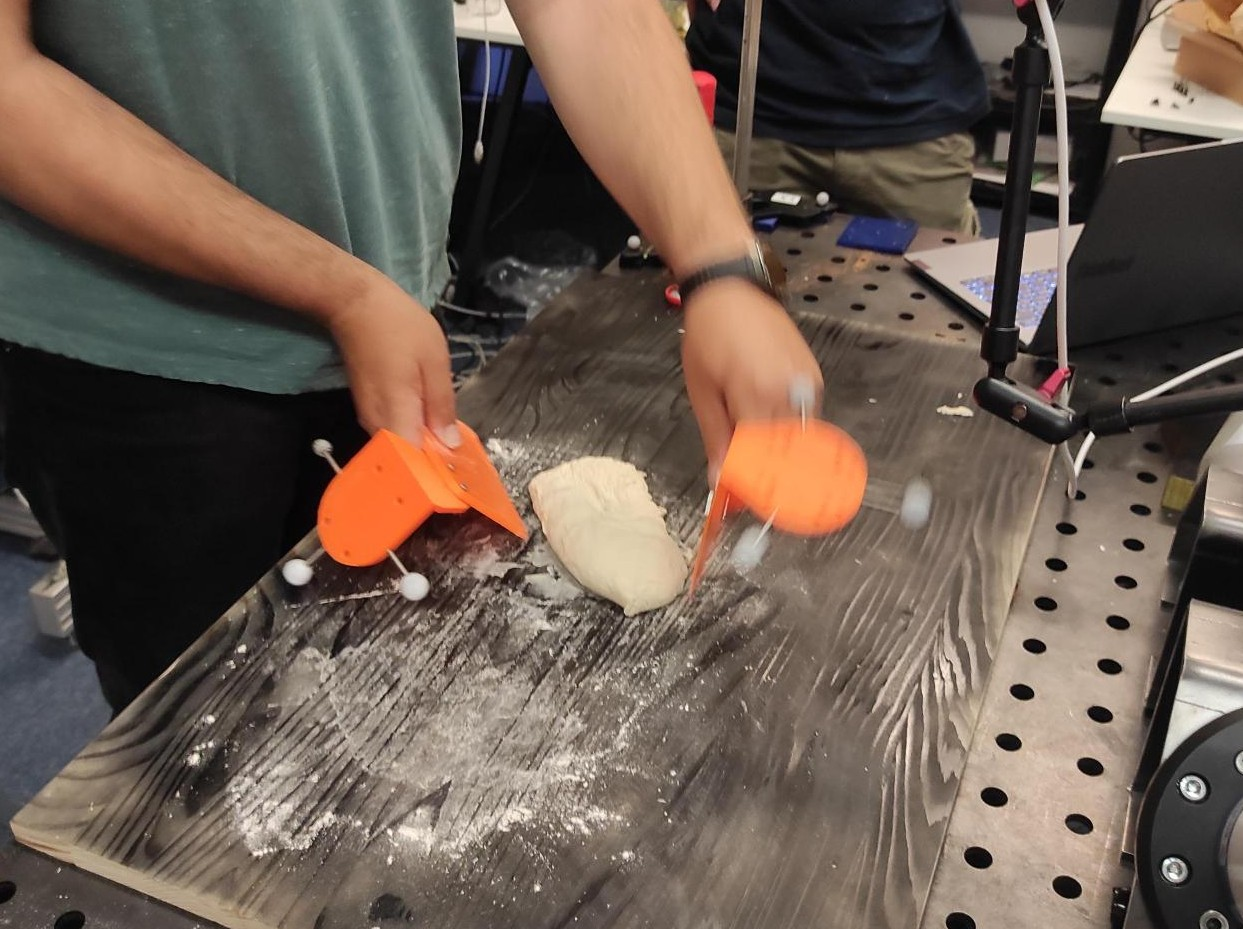
\includegraphics[width=\columnwidth]{figures/data_collection.jpeg}
    \caption{Operator shaping the dough into a ball using two spatulas during data collection. OptiTrack markers attached to the dough are visible.}
    \label{fig:data_collection}
\end{figure}

\subsection{Data Collection}

Data were collected using two 3D-printed spatulas. The experimental setup consisted of an Intel RealSense D435 camera and an OptiTrack motion-capture system. OptiTrack markers were attached to the spatulas to track their position and orientation during manipulation.

The transformation between the spatula mesh and the corresponding OptiTrack marker frame was determined through a calibration procedure using UR5e and Kinova Gen3 robotic manipulators. During calibration, a set of robot waypoints was recorded together with the corresponding marker poses measured by the OptiTrack system. These paired measurements were then used to estimate the transformation between the spatula mesh frame and the OptiTrack marker frame.